{
\setlength{\parindent}{2em}
\section{Black Box Symbol Access}\label{sec:das-mem-restore}
It was mentioned previously that, for integration reasons, the flight software code was considered unalterable (through requirement U02). Modifying the \gls{FSW} to accommodate the new checkpointing feature in BBPSim clearly defeated the purpose of encapsulation, and could potentially introduce errors in a critical piece of software. To represent reality as much as possible, the FSW was supposed to contain as fewer indications of the existence of \gls{BBPSim} as possible in its code.

In \autoref{sec:conditions}, it was shown that saving the entire set of statically-allocated variables in the DAS domain was a necessary condition for a stable restore. However, as it was forbidden to add \textit{getter} functions (e.g. \mintinline{c}|GetTheVariable()|) to access file-local variables from BBPSim, there needed to be a different solution. For the save and restore to be properly integrated, there needed to be a way to access them at runtime, a kind of indirect or "black box" access. 

In the end, the solution that was adopted involved the handling of DAS object files, \textit{after} they were compiled. Ultimately, no control over the flight software source code was given, but there was control over the compilation and building process. The following sections show how this limited control could be harvested, using a series of manipulations at build time, to give the \gls{BBPSim}-domain objects the required access to save the state of the flight software.

\subsection*{Linking Process}
First of all, it is crucial to understand how the linking process of an application is done. As mentioned earlier, when each source code file is compiled by \gls{GCC}, an \texttt{.o} object file is produced. For instance, let's take the code in \autoref{code:c-to-segments}. Although this file contains executable code, the object file that would be produced by GCC would, by itself, not be enough to be executable as a stand-alone. The \textit{linker} needs to first process the object files.

\begin{figure}[htbp]
	\centering 
	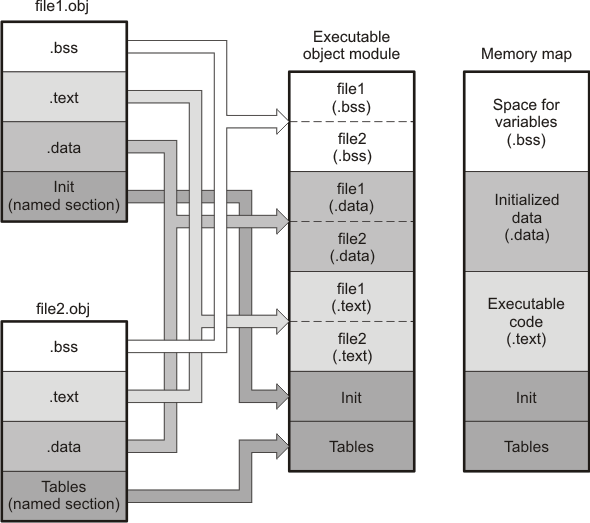
\includegraphics[width=.75\linewidth,keepaspectratio]{art/obj-to-elf-to-mem.png}
	\caption{Combining Input Sections to Form an Executable Object Module.\cite{online:linking}}
	\label{fig:link-mult-files}
\end{figure}

The linker's role in the building process is to combine each of the object files given as input into an executable file, or in the case of this thesis, a dynamic library. \autoref{fig:link-mult-files} better illustrates that concept. At linking time, the linker groups the same segments from each \texttt{.o} file together and lays them so in the executable object. Since the object file can be given in an arbitrary order, the linker can make no guarantee on the final layout.

In addition, while combining the object files together, the linker also resolves the undefined \textit{external} symbols, variables declared in one object file but used in another. 

Just like source code determines the resulting output of the compiler, it is also possible to control the linking process through the use of a linker script\cite{online:ld-scripts}. Even though, in most cases, users of the GNU linker don't provide a custom script, it is possible to specify one at linking time. 

Using such a script offers much more granularity to the developer in terms of which section gets put where in the executable object. In the field of embedded systems, this is particularly useful. Since certain components like non-volatile flash memory are adressable by the CPU, it lets the developer decide whether certain sections should be written to flash (e.g. addressed from 0x10000 to 0x50000) or just be allocated in RAM before running the program.

\begin{listing}[H]
	\vspace{12pt}
	\begin{minted}{c}
SECTIONS
{
	. = 0x10000;
	.text : { *(.text) }//$\label{line:link-ex}$
	. = 0x8000000;
	.data : { *(.data) }
	.bss : { *(.bss) }
}
	\end{minted}
	\caption{Simple example of a GNU ld linker script.}
	\label{code:link-script-ex}
\end{listing}

One can read the example linker script in \autoref{code:link-script-ex}  sequentially. On line \ref{line:link-ex}, the script lays out the \texttt{.text} sections of all the object files sequentially inside the executable object's own \texttt{.text} section, that starts at address 0x10000. Then, the linker does the same thing for the \texttt{.data} and \texttt{.bss} sections, starting at address 0x8000000.

\subsection*{Clustering Flight Software Sections}

- how to access everything (talk about dynamic library loading, elf dumps, double linking etc.)

\subsection*{Shared Object Considerations}\label{sec:dynlib-considerations}
- Dynamic library loading  https://eli.thegreenplace.net/2011/08/25/load-time-relocation-of-shared-libraries
- address at which the library is loaded (why always 0x00007fffXXXXXXXX?) https://unix.stackexchange.com/questions/509607/how-a-64-bit-process-virtual-address-space-is-divided-in-linux
In this case, application continerization is not possible, because we are a library.

}